\begin{frame}{Objectives of this study}
\begin{block}{Paper}
        \emph{Raissi, Maziar, Paris Perdikaris, and George E. Karniadakis. 2019. "Physics-informed neural networks: A deep learning framework for solving forward and inverse problems involving nonlinear partial differential equations." Journal of Computational Physics 378: 686-707. https://doi.org/10.1016/j.jcp.2018.10.045}
    \end{block}
\end{frame}

\begin{frame}{Introduction to Physics-Informed Neural Networks}
\begin{block}{}
        \emph{Physics-informed neural networks integrate deep learning with physical laws, enhancing robustness and predictive accuracy.}
    \end{block}
\begin{figure}[H]
    \centering
    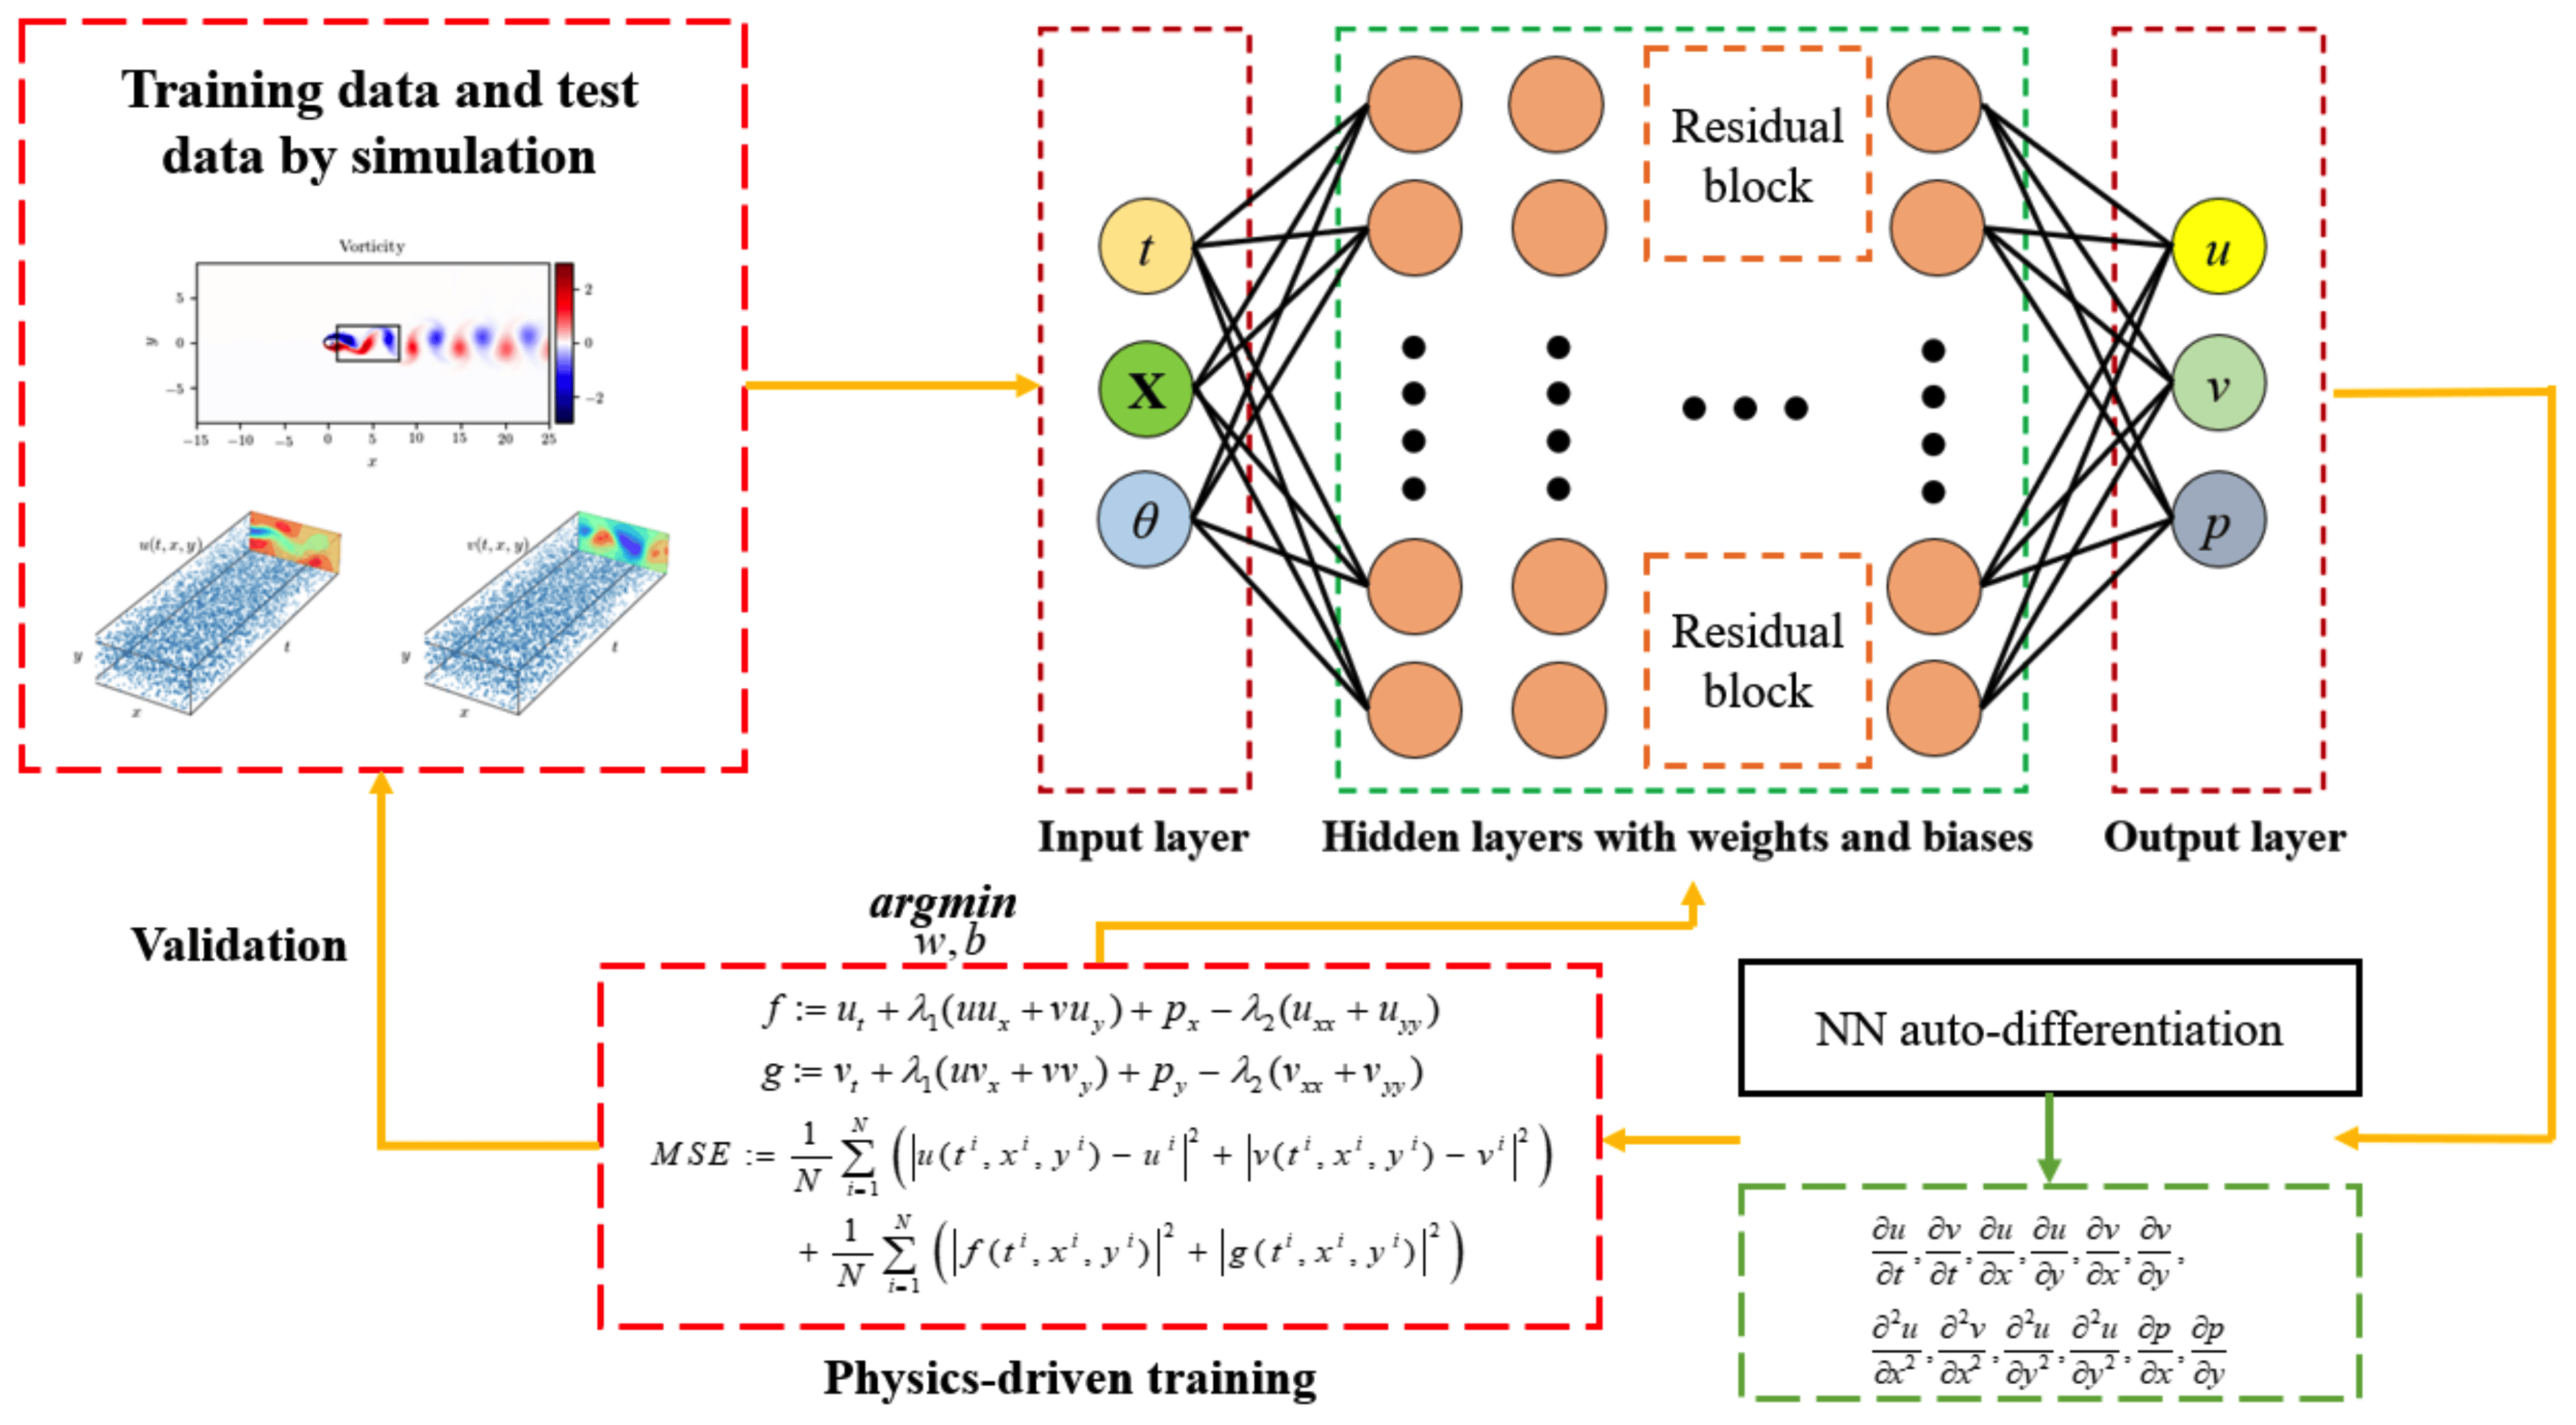
\includegraphics[width=0.8\textwidth]{img/pnn1.png}
    \caption{Schematic of a Physics-Informed Neural Network flow of data.}
    \label{fig:Physics-Informed Neural Networks}
\end{figure} 
\end{frame}

\begin{frame}{Key Components and Insights}
\begin{enumerate}
    \item \textbf{Versatility:} forward and inverse problems in systems described by nonlinear partial differential equations (PDEs)
    \item \textbf{Automatic differentiation (AD):} computation of derivatives up to any order without manual computation. 
    \item \textbf{Deep learning architecture:} facilitates the integration of differential equations directly into the loss function.
    \item \textbf{Computational efficiency:} Leveraging GPU acceleration and efficient training algorithms like L-BFGS (Limited-memory Broyden-Fletcher-Goldfarb-Shanno)
    \item \textbf{Generalizability across domains:} adaptable and can potentially be applied to a wide range of problems (finance, economics, and healthcare)
\end{enumerate}
\end{frame}

\begin{frame}{Theoretical Foundations of PINNs}
General formulation:
\[
u_t + \mathcal{N}[u; \lambda] = 0,
\]
where \( u(t, x) \) is the state variable representing the system's condition at time \( t \) and position \( x \), \( \mathcal{N} \) denotes nonlinear operators reflecting physical dynamics, and \( \lambda \) are parameters influencing these dynamics.
\begin{itemize}
  \item \textbf{Continuous Time Models}: The neural network models function \( u(t, x) \), trained to minimize the residual:
    \[
    f := u_t + \mathcal{N}[u] = 0
    \]
  \item \textbf{Discrete Time Models}: Implement numerical methods like Runge-Kutta for accurate time integration, enhancing model stability and accuracy.
\end{itemize}
\end{frame}

\begin{frame}{Evaluation}
\begin{block}{}
        \emph{Spatio-temporal solution and comparison across specific times.}
    \end{block}
\begin{figure}[H]
    \centering
    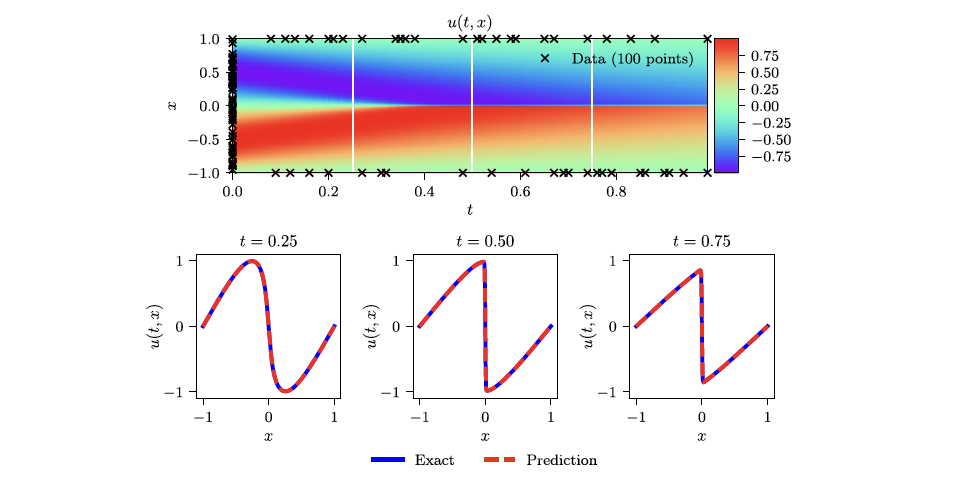
\includegraphics[width=0.8\textwidth]{img/Illustration2.png}
    \caption{Evaluation of PINN Predictions for a Nonlinear PDE.}
    \label{fig:Physics-Informed Neural Networks}
\end{figure} 
\end{frame}

\begin{frame}{Challenges with PINNs}
\begin{enumerate}
    \item \textbf{Sensitivity to hyperparameters:} layers, nodes, learning rates, method of numerical integration. 
    \item \textbf{Numerical stability and convergence:} automatic differentiation can cause problems (like with stochastic gradient descent)
    \item \textbf{Scalability and Computational Demands:} highlights computational intensity in training PINNs, especially with high-dimensional data.
    \item \textbf{Interpretability:} challenges of interpreting deep learning models in econometrics, crucial for understanding variable influences.
\end{enumerate}
\end{frame}

\begin{frame}{Potential Applications}
\textbf{Economics and Econometrics:}
\begin{itemize}
    \item Nonlinear Econometric Modeling
    \item Time Series Analysis
    \item Endogeneity and Instrumental variables
    \item Macroeconomic Modeling
    \item Real-Time Economic Policy Analysis
\end{itemize}
\textbf{Finance:}
\begin{itemize}
    \item Financial Markets
    \item Risk Management and Financial Stress Testing
    \item Portfolio Optimization
\end{itemize}
\end{frame}

\begin{frame}{Relevance to Econometrics}  
PINNs are used in complex econometric systems, particularly in nonlinear dynamics and sparse data scenarios.
\begin{itemize}
    \item \textbf{Model complex dynamics:} irregular data patterns or multi-factor interactions, where traditional models don't work (assumptions of linearity and normality).
    \item \textbf{Improve forecasting accuracy:} deep learning and economic axioms - for macroeconomic indicators and financial markets. 
    \item \textbf{Handle high-dimensional data:} for large numbers of financial instruments or economic indicators. 
    \item \textbf{Robustness for data quality:} reliable predictions in challenging data environments (noise, missing values, or anomalies). 
    \item \textbf{Prior knowledge}: integrate economic theories and constraints directly into the architecture, enhancing the credibility and theoretical consistency of model predictions.
\end{itemize} 
\end{frame}


